
The Public Health Initiative on Low- and Middle-Income Countries Air Pollution (PHILAP) is a study funded by the Medical Research Council that aims to study the health effects of air pollution in Delhi, India and other low- and middle-income countries, with a multidisciplinary team, including Data scientists and Social scientists. It will use RESpeck and Airspeck sensors to measure personal exposure to air pollution together with the stationary AIRSpeck while simultaneously measuring respiratory rate/flow and activity levels (with the RESpeck), to correlate this data with progress of respiratory diseases. This quantitative information will be allied with qualitative data such as the socio-geographic and cultural context of people's lives through the Social Sciences dimension of the study, for example with interviews with the participants, aiming to foster the dialogue between multiple disciplines to develop shared ways of analysing different types of datasets of air pollution.

The PHILAP pilot study, intended to reproduce in a smaller scale the deployment of these sensors and data collection techniques, as a trial for the bigger scale study in Delhi, India, where other studies are occurring with the same set of sensors, such as the Delhi Air Pollution: Health and Effects (DAPHNE) study. It also aims to engage with methodologies and challenges of working across distinct research methodologies.

The objective of this part of the project was to implement the requirements for the study from a technological point of view, recruit, organise and put into practice the data collection with participants. The task included the process of ethics approval by the School of Informatics following the data protection training course.

It is hoped that this data from the PHILAP study together with the online learning methods developed in this project will be employed in Part II of the Minf dissertation.

\section{Principles}

An application was developed by the Centre for Speckled Computing of The University of Edinburgh \cite{air-respeckapp} that connects to the sensors and records the values read into the smartphone's storage. However, that application did not include the capability of recording qualitative data such as photos, video, sound, and text. Those features were developed and integrated into the application that already existed. In addition, the User Interface was improved to allow easier access to the new features. The functional requirements for the features were:

\begin{itemize}
\item The user should be able to take a photograph, visualise and choose to save or discard that photograph.
\item The user should be able to record a video, visualise and choose to save or discard that video.
\item The user should be able to record an audio clip, reproduce it and choose to save or discard that clip.
\item The user should be able to save a text comment and save it.
\item All photographs, videos, audio recordings, and text comments should be time stamped for further analysis and synchronisation with other data (i.e., quantitative data).
\item The media collected should be saved in a folder inside the data collection folder to facilitate its upload to the servers along with the quantitative data collected.
\item The user should easily identify and select the data that they need to collect.

\end{itemize}

The following general principles of User Interface Design \cite{ui_design} were followed during implementation:

\begin{itemize}
    \item \textbf{Consistency, Aesthetically Pleasing, Predictability and Grouping:} The buttons created are consistent with the other buttons and grouped in their own section of the screen, indicating interactivity to the user. The format is familiar to the rest of the interface.
    \item \textbf{Directness, Clarity and Simplicity:} The user can access the function easily and complete a media collection cycle in three button presses: select type, capture and accept capture (except audio recording which requires four button presses). Buttons also become inactive if the action cannot be made at that moment.
    \item \textbf{Forgiveness, Control and Recovery:} The user has the control to review and accept or reject the media captured and is allowed to return to the main screen easily at any point of the media collection cycle.
\end{itemize}

\section{Implementation}

Figure \ref{fig:prototypes}, presents some prototypes designed to simulate the feature and facilitate discussion about the best way to implement this feature. As an output of the debate, given that the application is used in several countries such as the United Kingdom and India, with several different languages, it was opted to use icons instead of text to make the feature universally intuitive and usable (see Figure \ref{fig:main}). It was also essential to make the feature easily accessible, to decrease the difficulty for the users to collect data; therefore, the functionality was integrated into the subject mode screen of the application.

The features were developed in Android Studio using the Java programming language. The icons used were taken from Font Awesome, under CC BY 4.0 licence \cite{fontawesome}. 

\begin{figure}[H]
\begin{center}$
\begin{array}{lll}
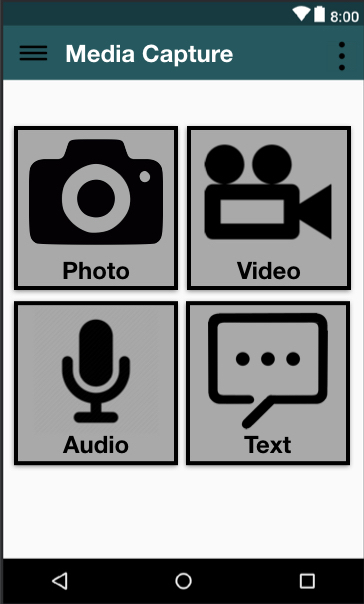
\includegraphics[width=.3\linewidth]{images/prototypes_001}&
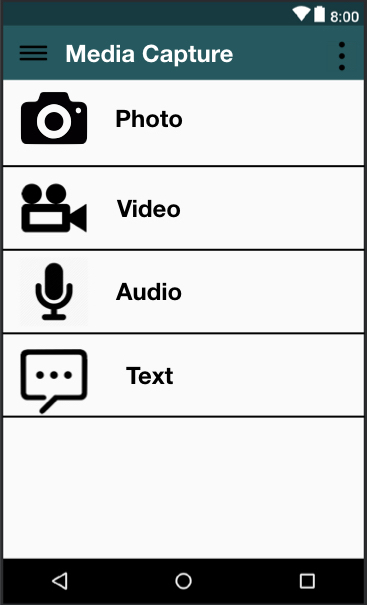
\includegraphics[width=.3\linewidth]{images/prototypes_002}&
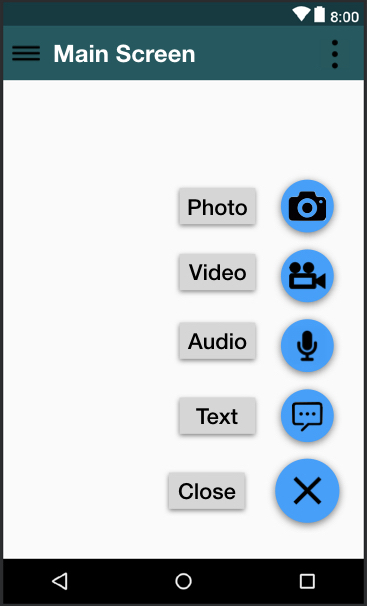
\includegraphics[width=.3\linewidth]{images/prototypes_003}
\end{array}$
\end{center}

\begin{center}$
\begin{array}{rr}
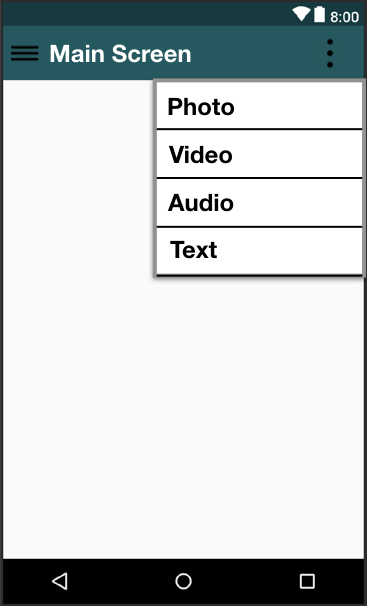
\includegraphics[width=.3\linewidth]{images/prototypes_004}&
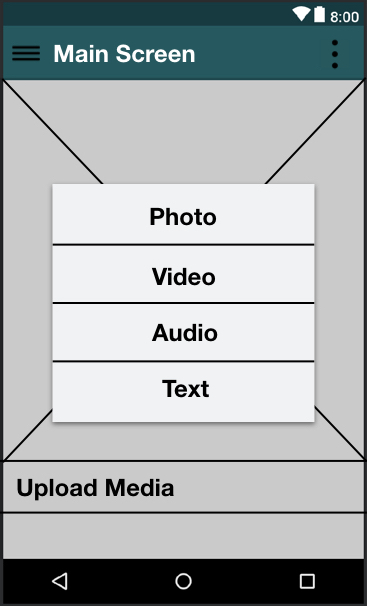
\includegraphics[width=.3\linewidth]{images/prototypes_005}
\end{array}$
\end{center}
\caption{Mock-ups of the feature}
\label{fig:prototypes}
\vspace{1cm}
\end{figure}


The final implementation included four buttons and their respective behaviour flow and is shown in Figure \ref{fig:main}. Each of the buttons intuitively indicates and launches a subsection of the feature: either the camera for photos and video recordings, the audio screen, shown in Figure \ref{fig:extras}, or the text comment dialog also shown in the same figure.

\begin{figure}[H] 
 
  \begin{minipage}[b]{0.5\linewidth}
    \centering
    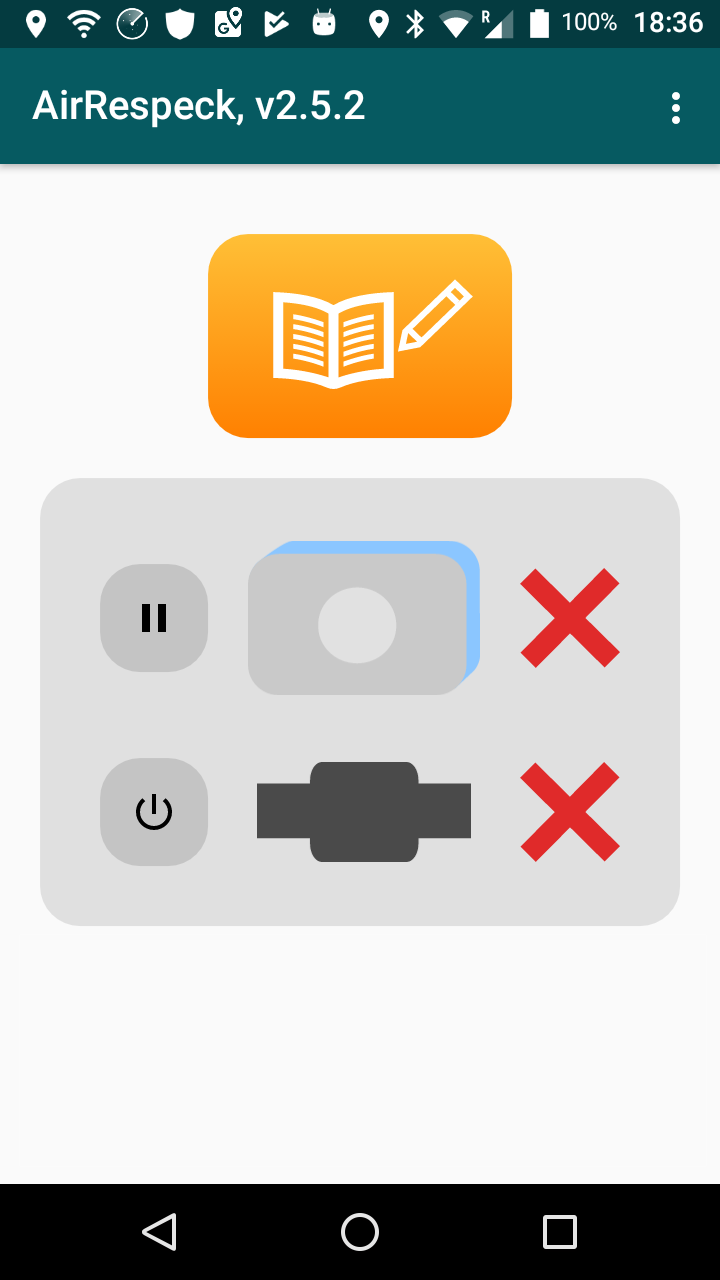
\includegraphics[width=.8\linewidth]{images/main_before} 
    \vspace{3ex}
  \end{minipage}%% 
  \begin{minipage}[b]{0.5\linewidth}
    \centering
    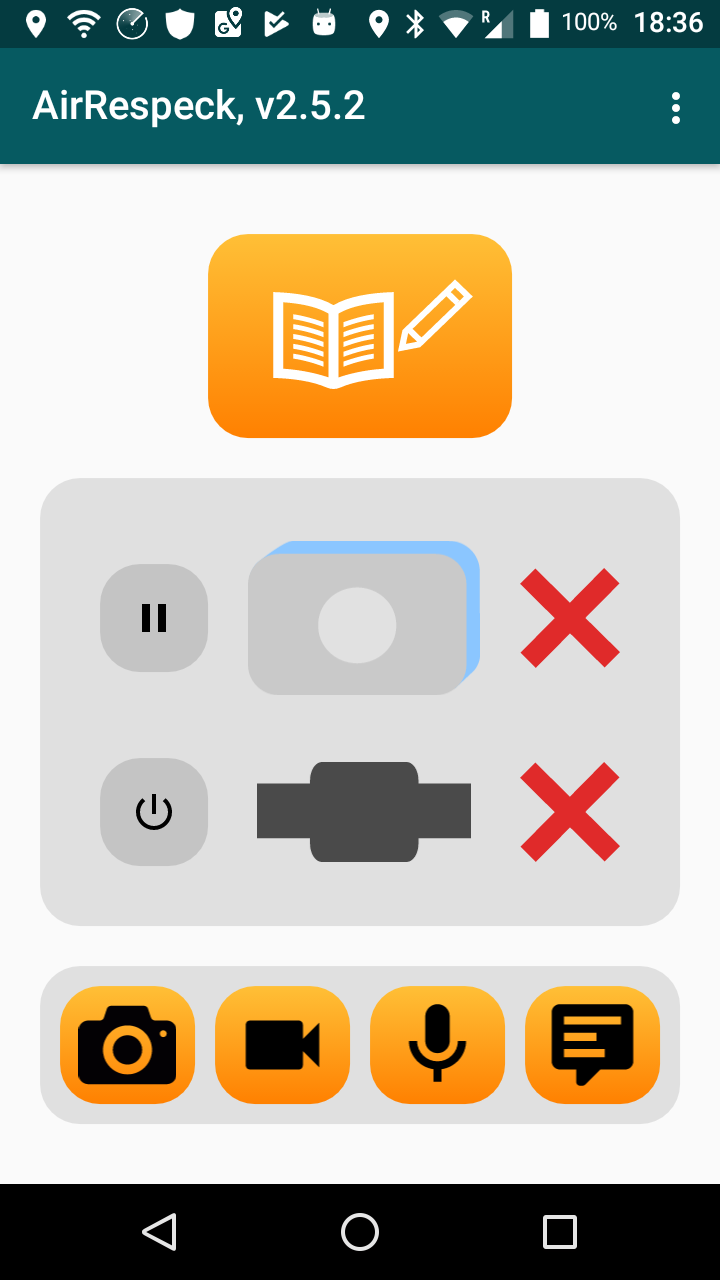
\includegraphics[width=.8\linewidth]{images/main} 
    \vspace{3ex}
  \end{minipage} 
  \caption{Subject mode before (left) and after (right) implementation }
  \label{fig:main}
  \vspace{0.5cm}
  \begin{minipage}[b]{0.33\linewidth}
    \centering
    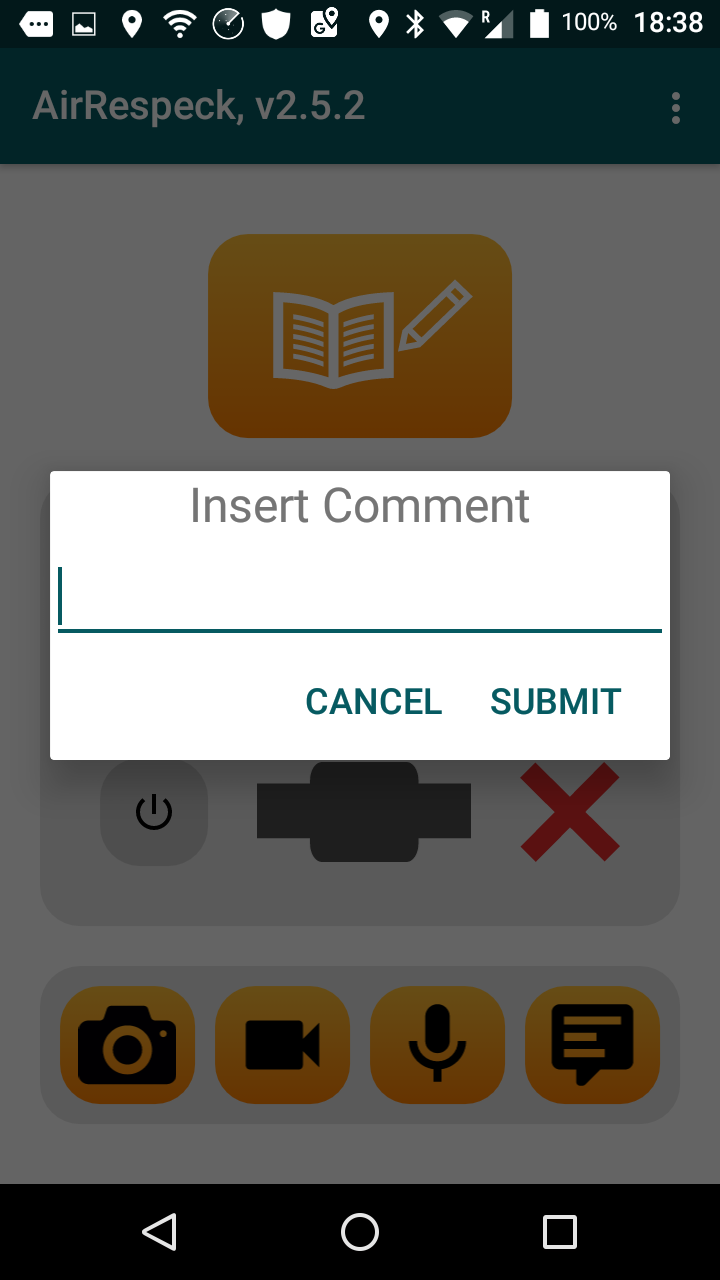
\includegraphics[width=.8\linewidth]{images/text} 
    \vspace{3ex}
  \end{minipage}%%
  \begin{minipage}[b]{0.33\linewidth}
    \centering
    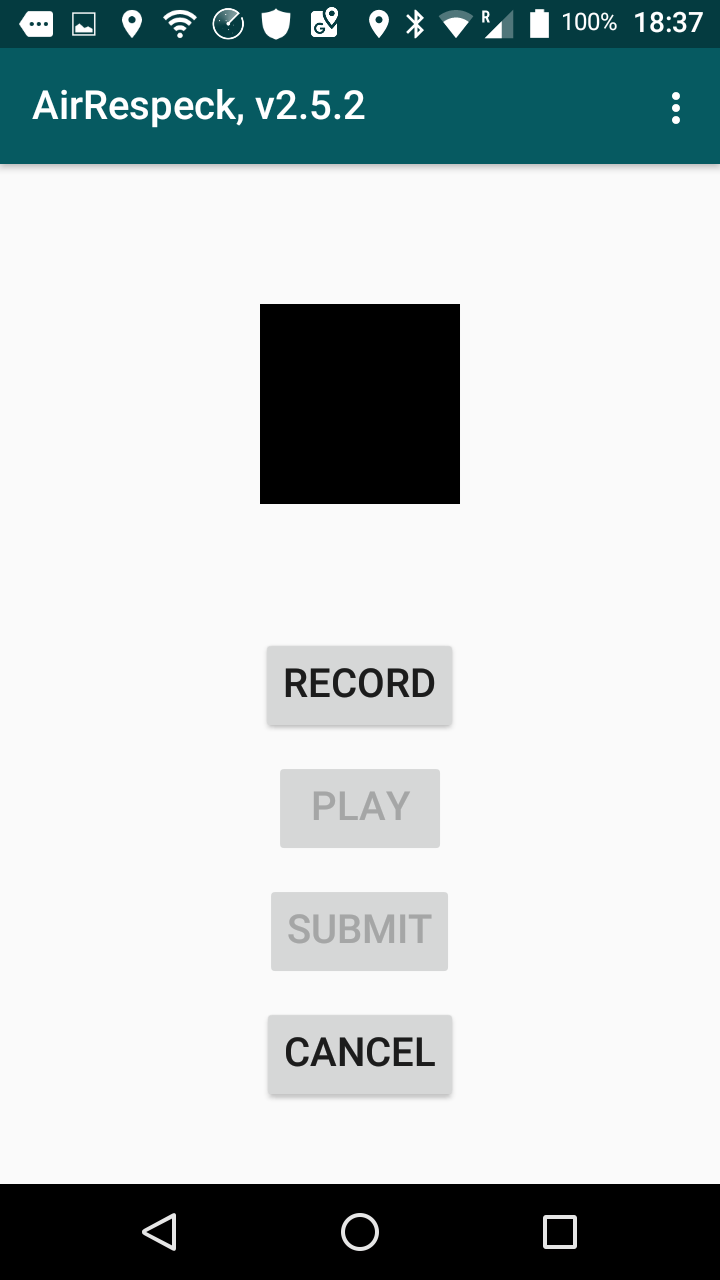
\includegraphics[width=.8\linewidth]{images/audio} 
    \vspace{3ex}
  \end{minipage}%%
  \begin{minipage}[b]{0.33\linewidth}
    \centering
    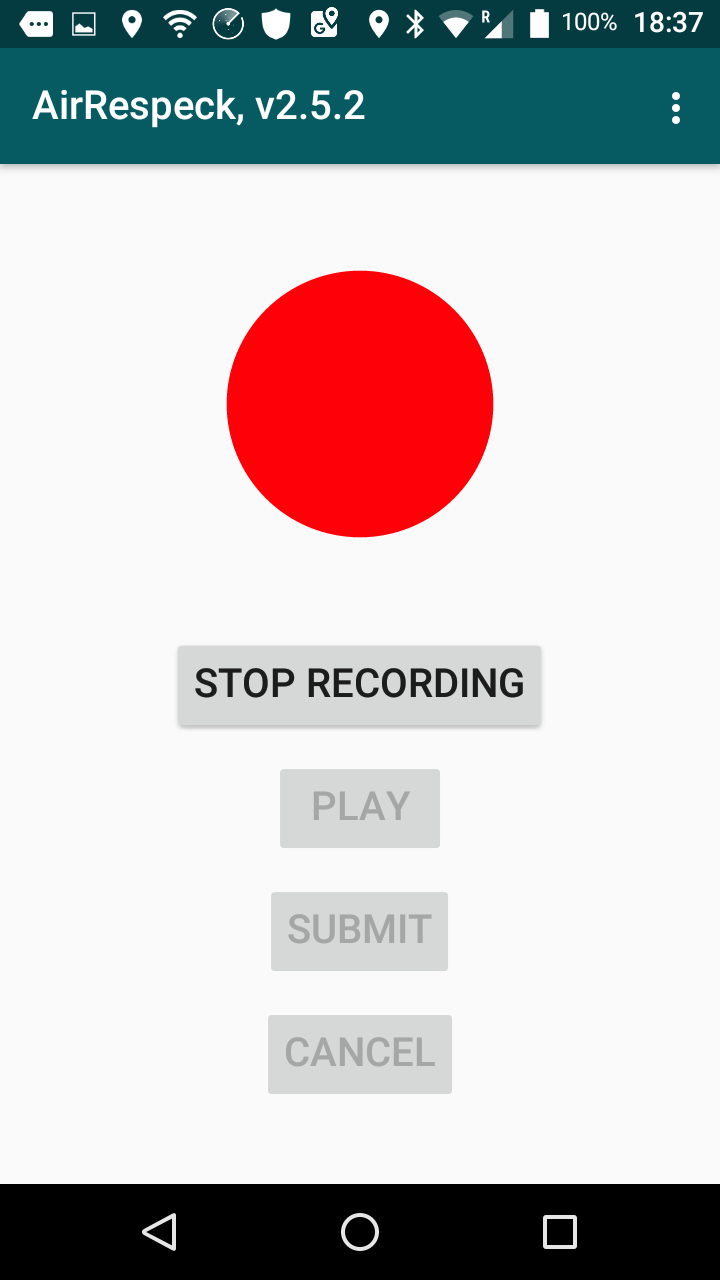
\includegraphics[width=.8\linewidth]{images/recording} 
    \vspace{3ex}
  \end{minipage} 
  \caption{Comment dialog (left), Audio Clip screen stopped (centre) and recording (right)}
  \label{fig:extras}

\end{figure}


\subsection{Data collection}
In order to be allowed to collect data from participants, an \textit{Information Sheet} was produced to provide to the participants in the pilot study. This document included all the details about the study and can be found in Appendix \ref{sec:infosheet}. The participants signed the School of Informatics' template for participation consent, presented in Appendix \ref{sec:consent}. 
To apply for ethics approval from the School of Informatics, the author studied an online data protection training course provided by the university and, in conjunction with the documents described above, obtained the approval to collect the data.
Students were asked to wear one AIRSpeck-P and a RESpeck sensor to collect breathing data and particulate matter in the environment. The RESpeck device was worn below the left rib, and the AIRSpeck was worn externally, like a belt. Students were provided with a phone connected to the sensors and were asked to observe and log information about air pollution and breathing sensations in the form of text, audio, photos or video clips, using the feature recently implemented.

\section{Results and analysis}

\subsection{Data visualisation}
A Python script was produced using Pandas \cite{pandas}, Matplotlib \cite{matplotlib}, Numpy \cite{numpy} and gmplot \cite{gmplot} to plot the air pollution and media collected data on a map and allowed to visualise the air pollution data collected with the participants and to incorporate the type of media used for collectioncollected into such visualisation. This program outputs, for every participant, an HTML file that lays on top of a map from Google Maps \cite{googlemapsapi}, circles with the air pollution readings coloured according to the value read and black markers that indicate the location of the media collected by the user. Hovering with the mouse on the black markers show the corresponding name of the file where such data was stored, allowing to connect the qualitative data to the quantitative data showed on the map. The fact that it is an HTML file with a Google Maps layer allows for the visualisation to be interactive with zoom and pan features. In addition, the program outputs an image with the legend of the circles' colours. An example of both outputs can be seen in Figures \ref{fig:map} and \ref{fig:scale} below.


\begin{figure}[H] 
\centering
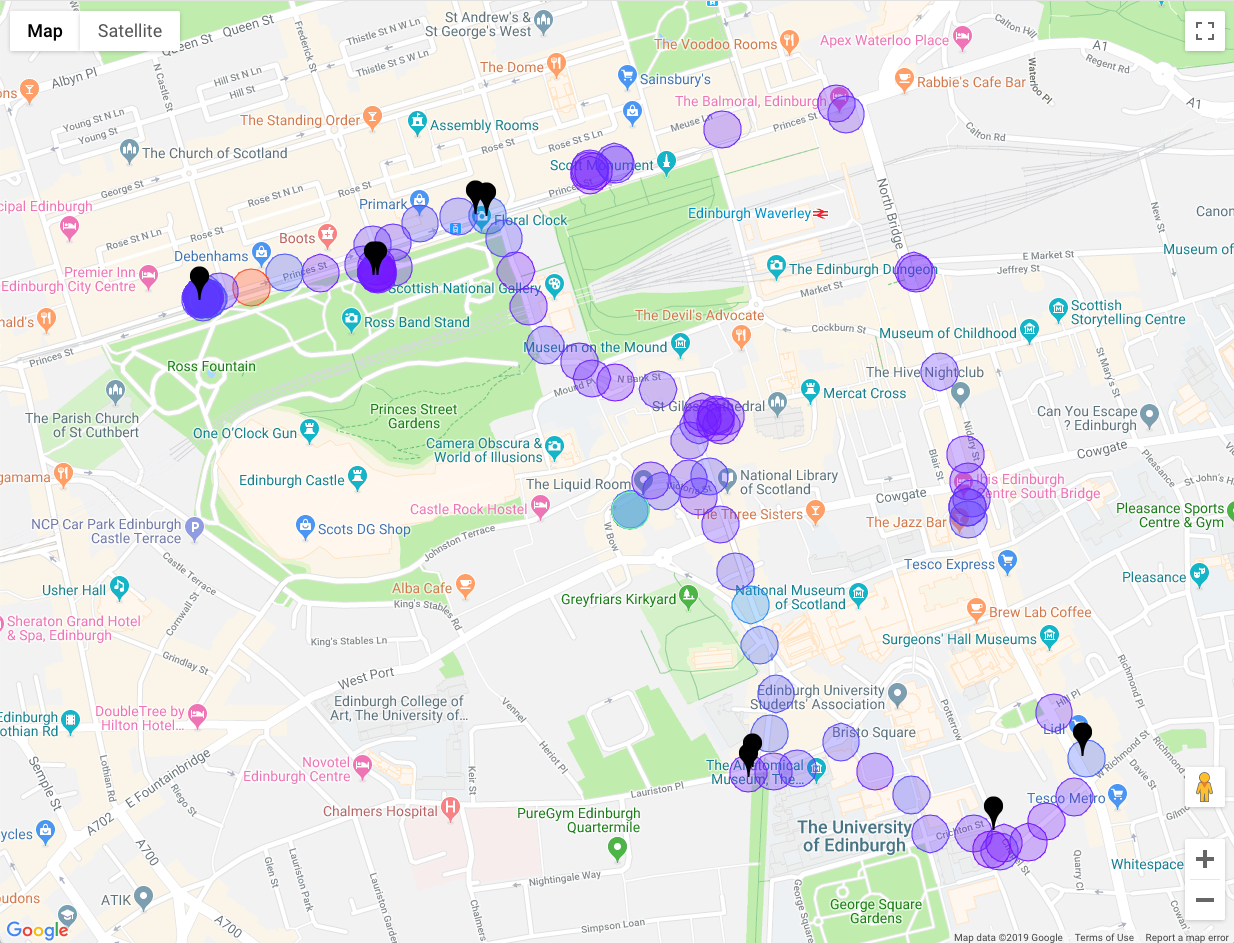
\includegraphics[width=\linewidth]{images/map_PHP001} 
\caption{Map and PM2.5 readings of Participant \#1}
\label{fig:map}
\vspace{0.5cm}
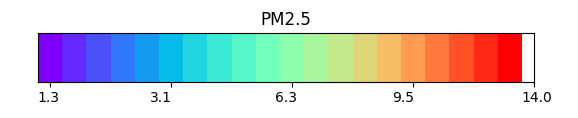
\includegraphics[width=.8\linewidth]{images/legend_PHP001} 
\caption{Legend corresponding to Participant \#1 PM2.5 data} 
\label{fig:scale}
\end{figure}


In the pilot study, ten people participated and collected data from two trips they performed in their daily routine: from home to work or university and vice-versa. During this period, they were asked to wear the AIRSpeck and RESpeck sensors and to use the media collection feature on the smartphone provided as they saw fit. Data collection took place between 10th October and 15th November 2018. Participant \#6 did not collect data correctly due to their misuse of the equipment.


Out of the 10 participants, 7 utilised the new media collection feature at least once. The feature was used a total of 41 times and Figure \ref{fig:mediacollected} shows a breakdown of the utilisation of the feature by media type. The most commonly used type of media collected and usually preferred was photos, followed by a similar number of text comments and video clips and lastly the least preferred option was audio clips which were used only three times.

\begin{figure}[H]
    \centering
    \begin{tikzpicture}
    \pie{44/Photos, 27/Text, 22/Video, 7/Audio}
    \end{tikzpicture}
    \caption{Breakdown of media collection by type}
    \label{fig:mediacollected}
\end{figure}

Each participant had different exposures to air pollution data. Some statistics were computed individually for each participant, presented below in Table \ref{tab:philapstats}. This information helps to interpret personal exposure of particulate matter. 

\begin{table}[H]
\centering
\resizebox{\textwidth}{!}{%
\begin{tabular}{l|cccc}
 & \textbf{\begin{tabular}[c]{@{}c@{}}Average PM1 \\ exposure\end{tabular}} & \textbf{\begin{tabular}[c]{@{}c@{}}Average PM2.5 \\ exposure\end{tabular}} & \textbf{\begin{tabular}[c]{@{}c@{}}Average PM10 \\ exposure\end{tabular}} & \textbf{\begin{tabular}[c]{@{}c@{}}Maximum PM2.5 \\ value read\end{tabular}} \\ \hline
\textbf{Participant 1} & 1.70 & 2.38 & 6.67 & 14.01 \\
\textbf{Participant 2} & 1.31 & 2.35 & 13.51 & 18.50 \\
\textbf{Participant 3} & 1.42 & 2.10 & 8.16 & 4.49 \\
\textbf{Participant 4} & 0.66 & 1.03 & 4.03 & 4.72 \\
\textbf{Participant 5} & 0.72 & 1.01 & 3.28 & 2.27 \\
\textbf{Participant 7} & 8.24 & 10.37 & 20.64 & 26.26 \\
\textbf{Participant 8} & 0.71 & 1.26 & 27.38 & 4.54 \\
\textbf{Participant 9} & 1.54 & 2.61 & 18.61 & 16.47 \\
\textbf{Participant 10} & 1.88 & 2.85 & 25.40 & 34.22
\end{tabular}%
}
\caption{Participants' statistics}
\label{tab:philapstats}
\end{table}

Interestingly, Participant \#7 measured unusually high values of PM2.5 exposure compared to other participants. The path that the participant took while collecting data can justify the high exposure values as the majority of the route was along a big construction site where a shopping centre was, being demolished and redeveloped, at the east end of Princes Street.

It is planned that in Part II of this project, data coming from the PHILAP project will be analysed in detail and converge with the online spatio-temporal models described in this project.